\chapter{Maloya : Un langage spécifique dédié aux services sensibles au contextes}\label{sec:dsl}
\begin{preamble}
Ce chapitre présente notre approche dédiée au domaine de l'assistance domiciliaire. Dans un premier
temps, nous décrivons l'architecture logicielle sous-jacente à notre approche. Ensuite, nous
introduirons un langage dédié pour développer des services sensibles au contexte
%\footnotemark{}\footnotetext{Ce travail à fait l'objet d'une soumission~:~\fullcite{carteron2017domain}.}
. 
\end{preamble}
\chpsummary{Contributions}
{
{\em Architecture logicielle} Un architecture qui couvre les besoins d'unification de données hétérogènes et d'exécuter des services en continu sur le flux d'évènements. ;
{\em Langage dédié} Un langage spécifique pour développer un large spectre de services sensibles au contexte, avec un haut niveau d'asbtraction et un traitement uniforme de sources de données hétérogènes.;
{\em Validation} redéfinition de 55 services, couvrant les besoins de tous les intervenants d'une plate-forme d'assistance pour le maintien à domicile de personnes âgées.
}

Sur la base de l'analyse de domaine présentée dans le chapitre précédent, 
nous somme en mesure de proposer un langage dédié aux services sensibles au 
contexte, appelé Maloya, ainsi que l'architecture logicielle sur
laquelle repose ce langage~:
\begin{itemize}
\item Notre architecture logicielle  est {\em centrée données}, en unifiant des sources 
hétérogènes de données, que ce soit en provenance de capteurs matériels ou de capteurs logiciels.
%fournir 
Elle fournit à l'ensemble des services une vue canonique des données mesurées. Ainsi, cette
forme canonique couvre d'une part, les
services de maintenance requérant l'état bas niveau des capteurs, et d'autre part, 
les services spécifiques aux aidants nécessitant des mesures d'activités de haut 
niveau. 
\item Le langage dédié Maloya fournit à la fois un cadre 
conceptuel et des outils pour concevoir et développer des services domiciliaires 
pour les personnes âgées. Notre langage est {\em orientée données} avec des services définis en 
terme de règles traitant des évènements et des états, et des opérateurs pour les combiner. 
%Pour unifier les source hétérogènes de données, des composants matériels aux 
%composant logiciels, notre approche promeut un paradigme ``centré données'' 
%et ``orienté données''. 
\end{itemize}

\section{Une approche dédiée au domaine de l'assistance domiciliaire}
Nous présentons ici les étapes principales de notre approche spécifique au domaine 
pour développer des services sensibles au contexte dédié au maintien à domicile 
des personnes âgées.

La fourniture d'un service sensible au contexte, selon notre approche, implique deux phases principales, illustrées en Figure~\ref{fig:functionalarchi}: 
\begin{itemize}
\item La phase de développement~: les intervenants définissent un service sous 
forme de règle en langage Maloya. Cette règle métier est ensuite compilée vers une règle de plus bas niveau en 
langage de traitement d'évènements. Les outils assistant le développeur de service lors de cette phase comprennent le 
compilateur et une interface de gestion des services.
\item La phase d'exploitation~: les services compilés sont exécutés sur les flux 
d'évènements provenant d'une maison sensible au contexte. Une fois mise en place, une règle est 
exécutée de façon à révéler chaque occurrence de la séquence d'évènements 
qu'elle décrit, jusqu'à ce que la règle soit supprimée, ou mise à jour. 
La phase d'exploitation est implantée par un analyseur d'évènements d'interaction qui 
transforme ces évènements en une forme canonique appelée {\em StreamEvent} 
(ou simplement, flux d'évènement, par la suite) pour alimenter un moteur de traitement d'évènements 
complexes (CEP). Ce moteur CEP est chargé de l'exécution des règles compilées sur le flux d'évènements.
%qui exécute les règles sur ce flux d'èvenements et retourner un signal lorsqu'une séquence d'évènements correspondant à une règle est identifiée dans le flux. 
\end{itemize}
\begin{figure*}[h]
\centering
  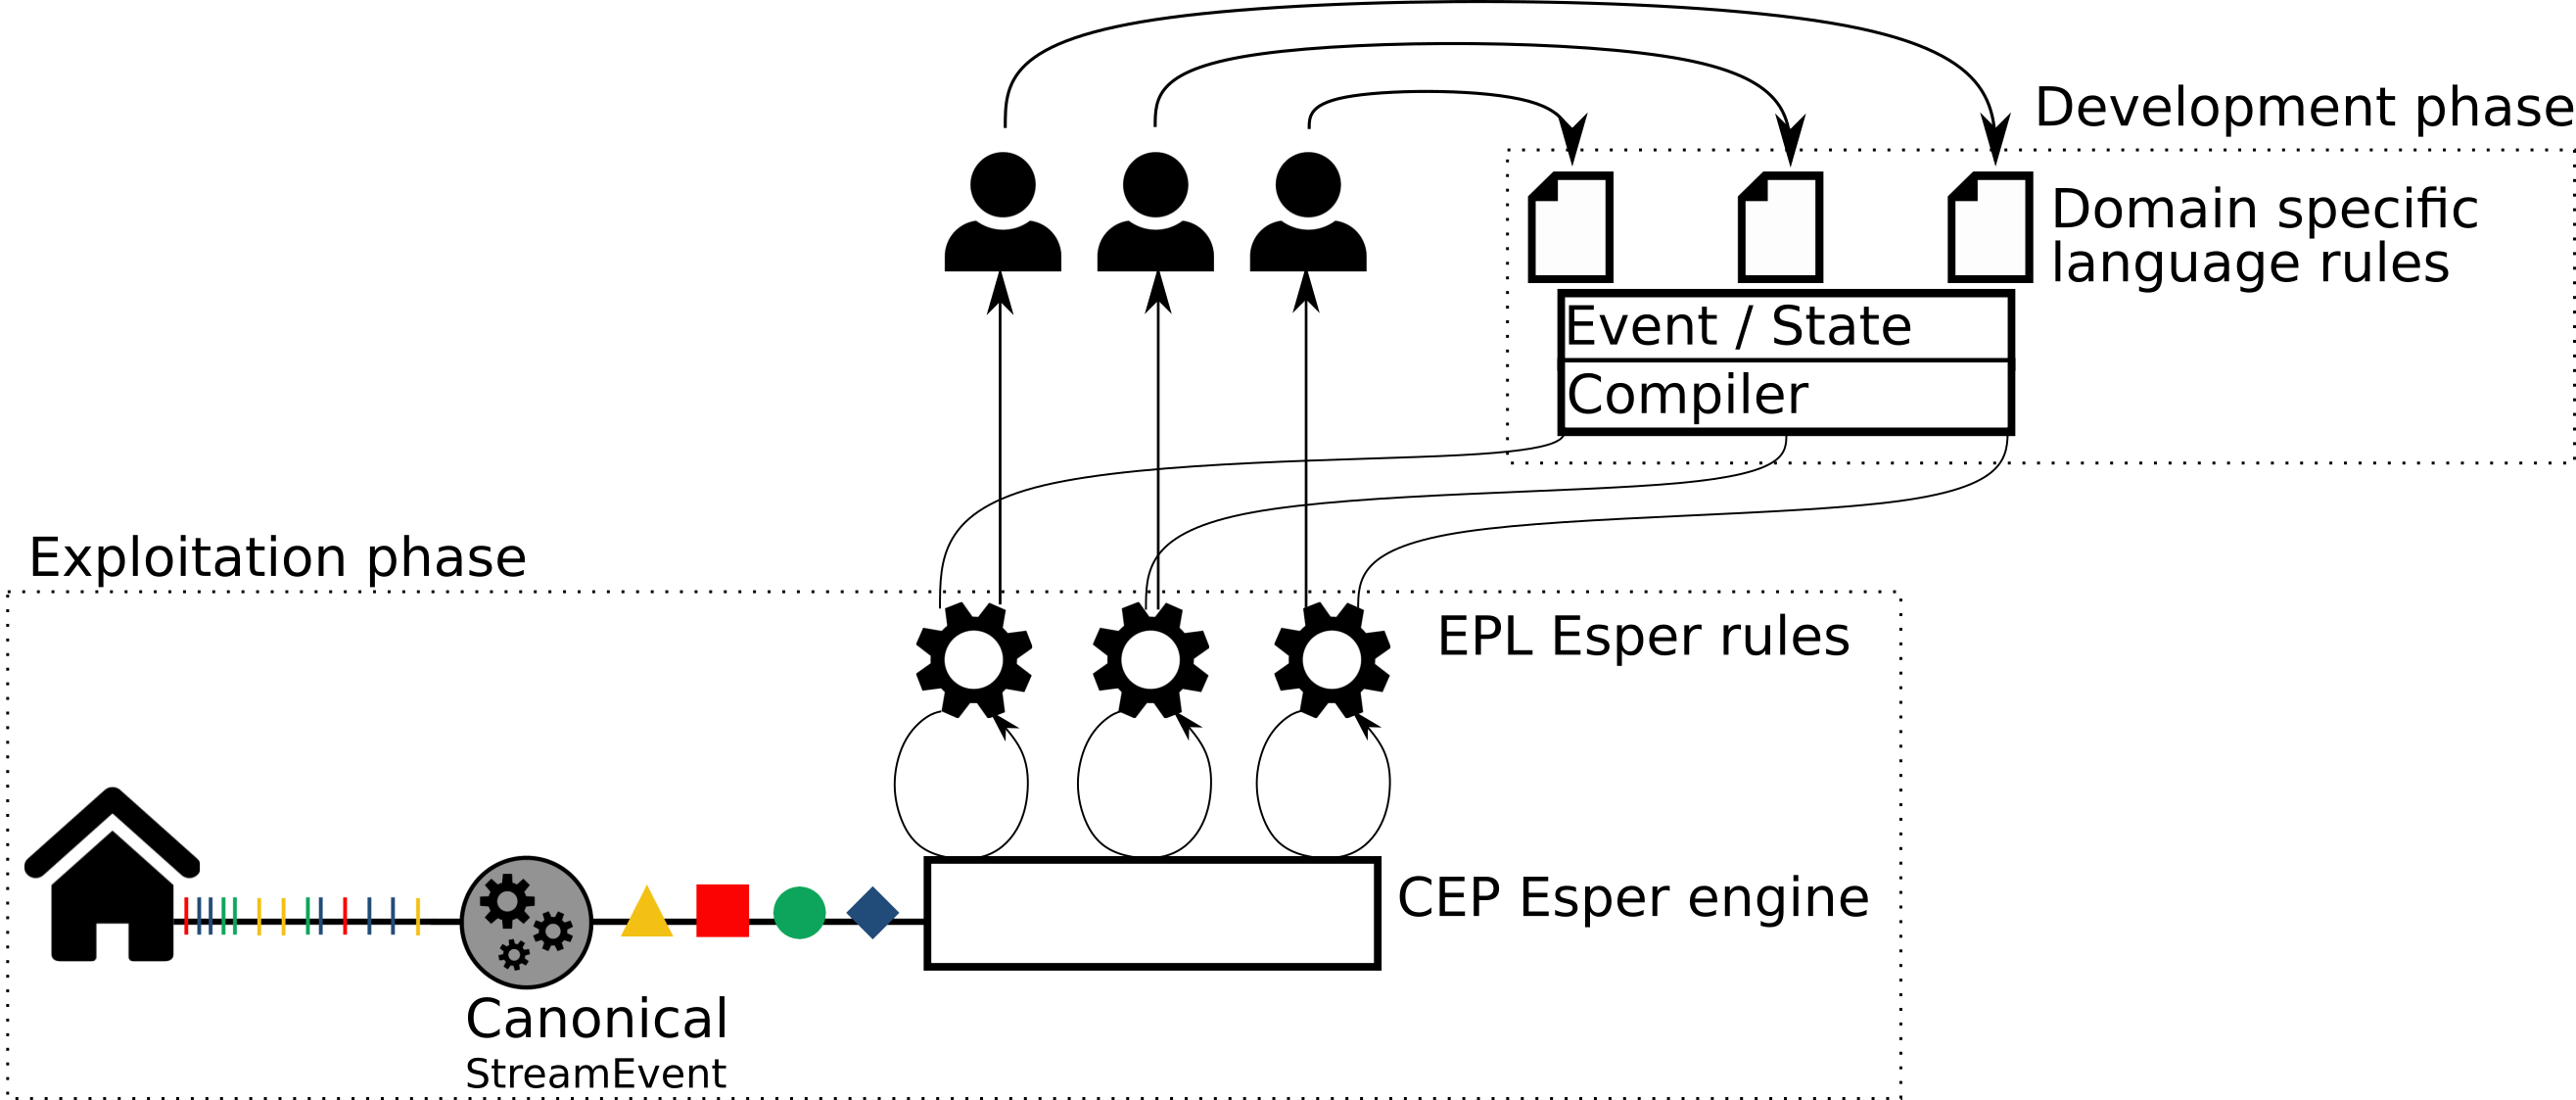
\includegraphics[width=\linewidth,totalheight=\textheight,keepaspectratio]{gfx/approach}
\caption{Vue globale de notre approche dédiée au domaine.}
\label{fig:functionalarchi}
\end{figure*}

\subsection{Définition du service}
La première étape est initiée par les intervenants qui expriment les scénarios 
de services. Ces scénarios sont soit directement écrits dans notre langage dédié par 
l'intervenant en exploitant les concepts d'états/évènements et les opérateurs 
de composition disponibles, si ils ont le bagage nécessaire, soit par un 
développeur de services, dans le cas contraire.
% dans le langage coeur

Notre implantation offre une interface graphique simple pour définir, compiler,
supprimer, et mettre à jour un service, 
comme illustré en Figure~\ref{fig:ui_rule}.
\begin{figure*}[h]
\centering
  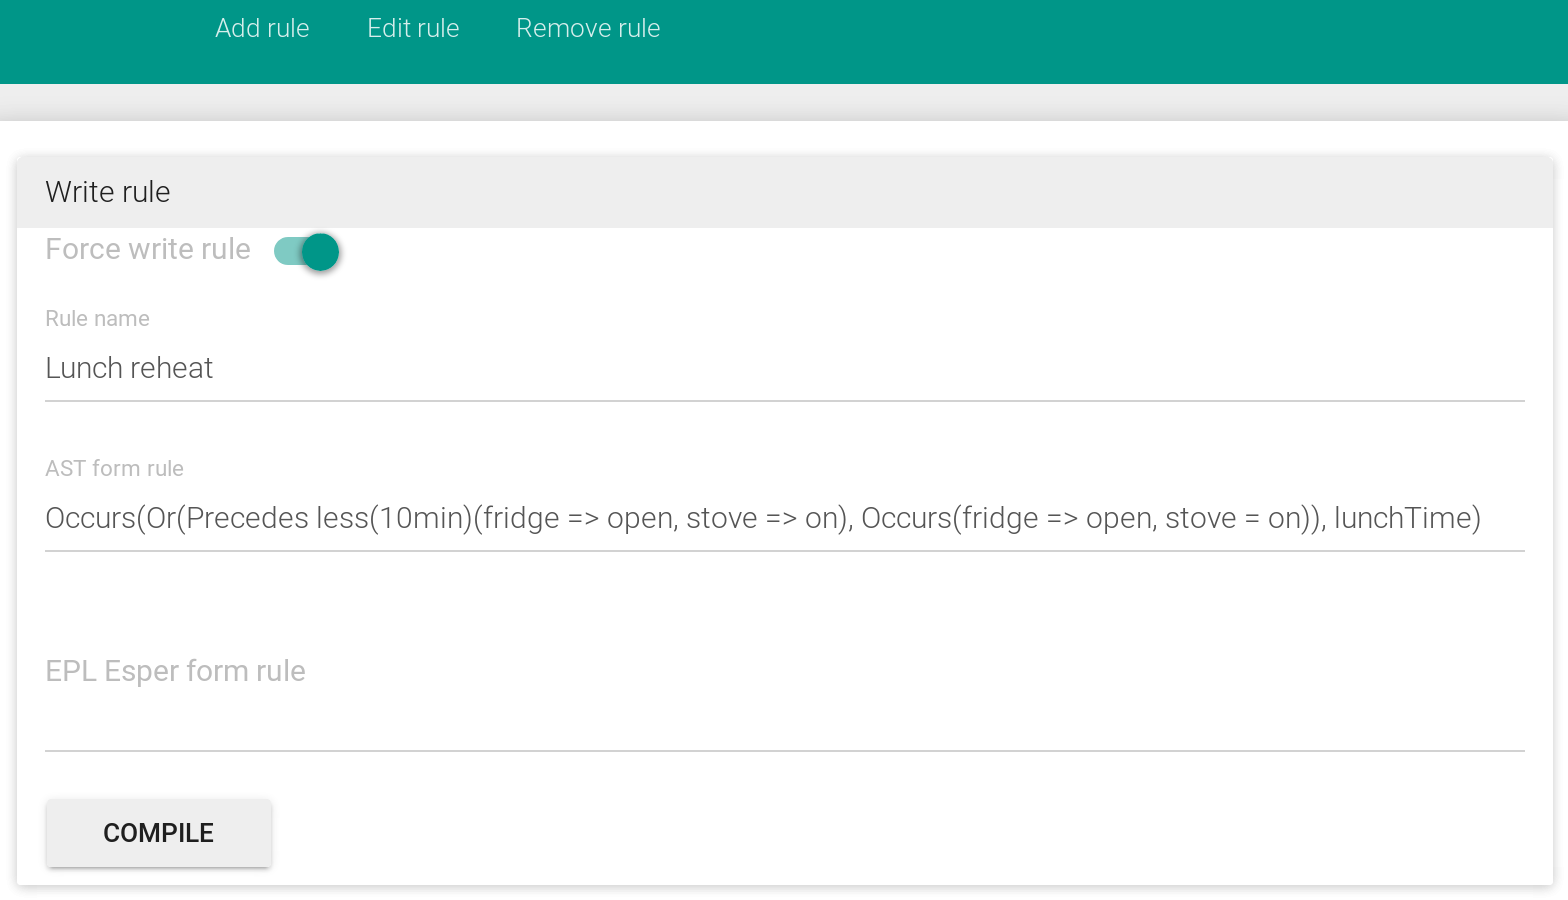
\includegraphics[width=\linewidth,totalheight=\textheight,keepaspectratio]{gfx/ui_add_rule}
\caption{Interface d'administration de service.}
\label{fig:ui_rule}
\end{figure*}

\subsection{Compilation du service}
Les services de haut niveau sont compilés vers un langage de traitement d'évènements qui exprime des règles de plus bas niveau. 
Le langage cible de traitement d'évènements ne supporte pas directement la notion d'état ainsi que nos opérateurs. Lors des étapes de compilation, ces concepts sont donc explicités sous forme de combinaisons d'évènements correspondants.

\subsection{Exécution du service}
Pour être déployées, les règles compilées sont enregistrées auprès du moteur CEP. Notre moteur d'exécution de règle est basé sur Esper, un CEP open-source développé par EsperTech\footnote{\url{http://www.espertech.com/esper/}}. 
Esper propose des interfaces Java et .Net avec NEsper, en tant que bibliothèques pour développer des programmes 
événementiels. Nous avons choisi Esper parce qu'il s'agit d'un moteur CEP 
populaire utilisé à la fois dans l'industrie et dans la recherche. Esper fournit 
un langage spécifique et déclaratif pour le traitement d'évènements complexes, 
appelé EPL (pour Event Processing Language). 
Ce langage inclut tous les opérateurs de SQL, et ajoute des constructions telles que la définition et l'interaction avec des fenêtres, ainsi que pour la génération de sorties.
EPL permet également de décrire des motifs 
d'évènements (ou ``Patterns'' EPL) à identifier dans un flux d'évènements temps réel, en utilisant des 
opérateurs pour ordonner les évènements, des contraintes temporelles, {\em etc.}. Ces opérateurs peuvent s'imbriquer
et permettent de définir explicitement la politique de sélection d'évènements avec la clause ``every''. 
Esper permet de recevoir les données en sorties d'une règle, soit en mode push, par l'utilisation de listeners, soit en mode pull, en utilisant des itérateurs.
%La seconde manière d'exprimer les motifs d'évènements utilise des expressions régulières. 
%Les deux syntaxes offrent la même expressivité.
% Esper propose des interface Java et C\# pour développer des programmes 
% événementiels. Nous avons choisi Esper parce qu'il s'agit d'un moteur CEP 
% populaire utilisé à la fois dans l'industrie et dans la recherche. Esper fournie 
% un langage spécifique et déclaratif pour le traitement d'évènements complexes, 
% appelé EPL (pour Event Processing Language). EPL permet de décrire des motifs 
% d'évènements à identifier dans un flux d'évènements temps réel, en utilisant des 
% opérateurs pour ordonner les évènements, des contraintes temporelles, {\em etc.} 
Cependant, Esper ne permet pas de manipuler le concept d'état, d'où la nécessité
d'encoder cette notion par des motifs purement évènementiels. 

\subsection{Forme canonique}
La forme canonique des données produites par un domicile sensible au contexte 
permet de traiter les mesures d'interaction indépendamment 
de leur format original. Cette forme canonique 
de données, nommée {\em StreamEvent}, est ainsi une couche d'abstraction sur l'hétérogénéité
des évènements des différentes sources, constituant un flux d'évènements uniforme. 
Dans cette représentation, chaque évènement est un 
quadruplet comprenant le type de l'évènement, sa localisation, sa valeur, et l'horodatage de son occurrence.

\[K\] (pour Kinds) est l'ensemble des types d'interactions (\eg Freezer)
\[L\] (pour Locations) est l'ensemble des localisation d'interactions (\eg Kitchen)
\[V\] (pour Values) est l'ensembles des valeurs de chaque domaine d'interaction (\eg open/close)
\[\mathds{N}\] est l'ensemble des horodatages (timestamps) d'instances d'interactions
\[
  v \in \mathds{V} \in \overset{m}{\underset{j=0}\cup}D_{K_i}
\] 
\[ 
t \in \mathds{N}
\]
in
\[
  s \in S=\mathcal{P}(K\times L\times \mathds{V}\times \mathds{N})
\]
\[
  s =\{(k_0,l_0,v^{D_{k_0}}_0,t_0), \dots, (k_n,l_o,v^{D_{k_n}}_n,t_n)\}
\]

Notons que le flux d'évènements en format StreamEvent ainsi défini est plus bas niveau que
le format des rôle défini en Section~\ref{archi:algebra}. En effet, comme dans les langages de CEP, utilisés comme cible,
les évènements sont toujours ponctuels (\ie n'ont pas de durée)\footnote{Même
dans les langages CEP avec une sémantique d'intervalle, les évènements élémentaires
sont toujours ponctuels, comme discuté en Section~\ref{sec:cep}.}, nous ne pouvons pas réutiliser
directement les évènements de rôles, qui étaient estampillés par des intervalles de temps (les périodes).
En revanche, ce nouveau format permet de détecter de manière plus précoce certains évènements
complexes, sans attendre la fin d'un évènement, pouvant avoir une durée non négligeable. Par exemple,
prenons la règle vérifiant si une porte reste ouverte pendant plus de 3 heures. Avec un log
d'évènements de rôles, cette règle ne pouvait déclencher que lorsque la porte était refermée,
car c'est à ce moment-là que l'évènement ``interaction de porte'' se produisait. Au contraire,
avec un log en format StreamEvent, il devient possible d'observer l'ouverture de porte indépendamment
de sa fermeture, et donc de réagir, en principe, dès que le délai de 3 heures s'est écoulé. Nous
verrons par la suite comment notre langage dédié atteint effectivement cette réactivité en
s'appuyant sur le langage cible Esper. Ce niveau de réactivité n'était pas capital dans le contexte
du Chapitre~\ref{cha:fiabilite}, où le signalement à la volée des dysfonctionnements des capteurs 
servait au service de maintenance, ayant un cycle d'intervention de l'ordre de plusieurs jours. Il en
est tout autrement dans le contexte du chapitre actuel où l'on s'intéresse à une classe bien plus large de services,
incluant des assistances de sécurité et des rappels d'activités.


\section{Langage de règles}

Le langage Maloya fournit une base d'expressions contraintes
permettant d'exprimer l'ensemble des services nécessaires à
l'assistance domiciliaire des personnes âgées.  Ce langage permet aux
intervenants de définir des services plus simplement que par des
langages de programmations conventionnels.  En effet, il restreint son
expressivité aux seuls concepts nécessaires au domaine des services
sensibles au contexte pour l'assistance domiciliaire. Pour ce faire,
Maloya rend explicite les notions d'évènements, d'états et les
opérateurs de composition.  

Les intervenants peuvent définir les scénarios correspondant à un
service à travers des règles constituées simplement par des
compositions d'évènements et/ou d'états.  En outre, à cause de la
nature récurrente des services relatifs à l'assistance domiciliaire
(\eg les activités quotidiennes telles que les repas ou la toilette),
une règle est conçue pour que son exécution détecte chaque occurrence
de la composition qu'elle décrit.

Il existe deux représentations du langage~; une représentation interne,
qui constitue la représentation de base de notre langage, et une représentation
textuelle qui permet d'exprimer des règles sous forme d'une phrase en
langage naturel contraint.  Il est important de noter que les
représentations internes et textuelles de notre langage sont
parfaitement équivalentes~: la représentation textuelle étant simplement une
formulation plus naturelle des expressions définies dans la
représentation interne.

\section{Évènements et États}\label{sec:dsl:eventstate}
Notre langage est construit autour de l'expression d'évènements et d'états. 
Un évènement est exprimé ainsi~: 
\begin{lstlisting}[language=MaloyaText]
p becomes v
\end{lstlisting}
% en langage textuel. 
Un état est exprimé comme suit~: 
\begin{lstlisting}[language=MaloyaText]
p is v
\end{lstlisting}
%en langage textuel. 
Dans chaque cas, {\tt p} est l'identification d'une interaction
(matérielle ou logicielle) et {\tt v} appartient à l'ensemble des
valeurs possibles pour l'interaction considérée. L'évènement {\tt p
  {\em becomes} v} survient quand la mesure de l'interaction {\tt p}
signale une valeur {\tt v}, si sa précédente valeur était
différente. L'état {\tt p {\em is} v} commence précisément quand
l'évènement {\tt p {\em becomes} v} se produit~; il se termine quand
l'évènement {\tt p {\em becomes} v'} se produit, où {\tt v'} $\neq$
{\tt v}. Nous voyons la période durant laquelle un état se maintient
comme l'{\em intervalle de temps} d'un état.
%Cette notion est généralisée pour les évènements en les considérant comme des intervalles de temps nuls. 
%NV: a-t-on besoin de considérer un event comme un état de longueur nulle? Je pensais qu'au contraire,
%les opérateurs demandant un état n'acceptent pas un event!

La notion d'intervalle de temps est utilisée pour définir les
opérateurs et leur sémantique. La Figure~\ref{fig:event_state}
présente la syntaxe et la sémantique informelle des évènements et
états.  Un évènement est représenté comme une pointe de signal.
% avec ses points de départs et de fin fusionnés.
Un état est représenté par un signal rectangulaire~; ses points de
départ et de fin correspondent à l'occurrence d'évènements provoquant
son début et sa fin.

\begin{figure}[h]
  \begin{footnotesize}
    % \begin{center}
    \begin{tikzpicture}[node distance=\dx and \dy,
      >=latex,shorten >=2pt,shorten <=2pt,auto,
      semithick,initial distance=1cm,
      every initial by arrow/.style={*->} ]
      \draw[gray!50,line width=0.1mm,dashed] (-1.5,.5) -- (-1.5,-1.2);
      \draw[gray!50,line width=0.1mm,dashed] (1.5,.5) -- (1.5,-1.2);  
      \draw[gray!50,line width=0.1mm,dashed] (-.5,.2) -- (-.5,-1.);
      \draw[gray!50,line width=0.1mm,dashed] (.5,.2) -- (.5,-1.);  
      \draw[] (-1.5,.) 
      node[xshift=-3 cm,yshift=.125cm] { Event~:} 
      node[xshift=-1.5 cm,yshift=.3cm] { {\tt p {\em becomes} v}} 
      node[xshift=-1.5 cm,yshift=. cm] { $p\Rightarrow v$} 
      node[xshift=-.2 cm,yshift=0 cm] { {\tt e}} --(-.5,.)--(-.5,.4) -- (-.5,.) -- (1.5,.);
      \draw[] (-1.5,-.6) 
      node[xshift=-.12 cm,yshift=.25cm] { ${\tt v}$} 
      node[xshift=-.1 cm,yshift=. cm] { ${\tt v'}$} 
      node[xshift=-.25 cm,yshift=.125 cm] { {\tt p}} -- (-.5,-.6) -- (-.5,-.2) -- (.5,-.2) -- (.5,-.6) -- (1.5,-.6);
      \draw[] (-1.5,-1.2) 
      node[xshift=-3 cm,yshift=.125cm] { State~:} 
      node[xshift=-1.5 cm,yshift=.3cm] { {\tt p {\em is} v}} 
      node[xshift=-1.5 cm,yshift=. cm] { $p=v$} 
      node[xshift=-.2 cm,yshift=0 cm] { {\tt s}} -- (-.5,-1.2) -- (-.5,-.8) -- (.5,-.8) -- (.5,-1.2) -- (1.5,-1.2);
    \end{tikzpicture}
  \end{footnotesize}
  \caption{Semantique informelle et syntaxe des état et évènement.}
  \label{fig:event_state}
\end{figure}

Les états disposent également de filtres sur leur durée.  Ces filtres
permettent de borner la période d'un état avec une limite haute ou une
limite basse. La limite haute de la durée d'un état est exprimée
ainsi~:
\begin{lstlisting}[language=MaloyaText]
p is v less than t
\end{lstlisting}
et la limite basse est exprimée comme suit~:
\begin{lstlisting}[language=MaloyaText]
p is v for at least t
\end{lstlisting}
où {\tt t} représente une période de temps.

\section{Les opérateurs}\label{sec:dsl:operator}
Une {\em règle} dans notre langage est constituée d'opérateurs manipulant les 
états et/ou les évènements. Tous les opérateurs retournent des évènements.
Plus précisément, un opérateur produit un évènement de succès quand le contexte 
décrit par l'application de l'opérateur à des états/évènements est détecté.
Puisqu'un opérateur retourne un évènement, les opérateurs qui prennent en argument un évènement
peuvent prendre également une application d'opérateur comme argument.
En revanche, les opérateurs qui prennent un état comme argument ne peuvent 
pas prendre une application d'opérateur comme argument.
L'imbrication des opérateurs n'est ainsi pas arbitraire et suit notre étude de domaine.

La Figure~\ref{fig:operators} présente la double syntaxe des
opérateurs de notre langage (représentation interne et textuelle),
ainsi que sa sémantique informelle.  La syntaxe est présentée sur la
partie gauche. Sur la partie droite, une représentation graphique,
suggère la sémantique de l'opérateur comme une fonction booléene
définie sur le temps.  Cette représentation permet de visualiser les
évènements et les états impliqués dans une application d'opérateur, et
la façon dont les opérateurs les combinent.
%Chaque construction en langage textuelle est complétée de sa construction équivalente en langage c\oe ur.
% example greater less
%variant : precedes less, precedes greater

%\end{center}
 % \begin{multicols}{2}
\begin{figure*}[!h]
\begin{footnotesize}
\begin{tikzpicture}[node distance=\dx and \dy,
      >=latex,shorten >=2pt,shorten <=2pt,auto,
      semithick,initial distance=1cm,
      every initial by arrow/.style={*->} ]   
      \draw[gray!50,line width=0.1mm,dashed] (-1.5,.5) -- (-1.5,-1.2);
      \draw[gray!50,line width=0.1mm,dashed] (1.5,.5) -- (1.5,-1.2);  
      %%%%%%%%%%%%%%%%%%%%%%%%%%%%%%%%%%%%%%%%%%%%%%%%%%%%%%%%%%%%%%%%%%%%%%%
      \draw[gray!50,line width=0.1mm,dashed] (.5,.) -- (.5,-1.2);   
      \draw[] (-1.5,.) 
      node[xshift=-.25 cm,yshift=.125cm] {{\tt e$_1$}}  --(-.5,.)--(-.5,.4) -- (-.5,.) -- (1.5,.);
      \draw[] (-1.5,-.6) 
      node[xshift=-.25 cm,yshift=.125cm] {{\tt e$_2$}} -- (.5,-.6) -- (.5,-.2) -- (.5,-.6) -- (1.5,-.6);
      \draw[] (-1.5,-1.2) 
      node[xshift=-4.1 cm,yshift=1.cm] {Every time {\tt e$_1$} {\em immediately} precedes {\tt e$_2$}}
      node[xshift=-3. cm,yshift=.25cm] {{\tt e$_1$ {\bf precedes} e$_2$ $\Leftrightarrow$ $Precedes(e_1,e_2)$}}
      node[xshift=-1.5 cm,yshift=-.45cm] {Variants:}
      node[xshift=3.5 cm,yshift=-.3cm] {{\tt e$_1$ {\bf precedes within} t e$_2$ $\Leftrightarrow$ $Precedes\_less(t)(e_1,e_2)$}}
      node[xshift=3.45 cm,yshift=-.65cm] {{\tt e$_1$ {\bf precedes by} t e$_2$ $\Leftrightarrow$ $Precedes\_greater(t)(e_1,e_2)$}} -- (.5,-1.2) -- (.5,-.8) -- (.5,-1.2) -- (1.5,-1.2);
      %%%%%%%%%%%%%%%%%%%%%%%%%%%%%%%%%%%%%%%%%%%%%%%%%%%%%%%%% 
      \draw[gray!50,line width=0.1mm,dashed] (-1.5,-2.) -- (-1.5,-3.7);
      \draw[gray!50,line width=0.1mm,dashed] (1.5,-2.) -- (1.5,-3.7);  
      \draw[gray!50,line width=0.1mm,dashed] (-.5,-2.5) -- (-.5,-3.7);   
      \draw[gray!50,line width=0.1mm,dashed] (.,-2.5) -- (.,-3.7);  
      \draw[gray!50,line width=0.1mm,dashed] (.5,-2.5) -- (.5,-3.7);
      \draw[] (-1.5,-2.5) 
      node[xshift=-.25 cm,yshift=.125cm] {{\tt e}} --(-.5,-2.5)--(-.5,-2.1)--(-.5,-2.5)--(.,-2.5)--(.,-2.1)--(.,-2.5)--(.5,-2.5)--(.5,-2.1)--(.5,-2.5) -- (1.5,-2.5);
      \draw[] (-1.5,-3.1) 
      node[xshift=-.25 cm,yshift=.125cm] {{\tt s}} -- (-1,-3.1) -- (-1,-2.7) -- (1,-2.7) -- (1,-3.1) -- (1.5,-3.1);
      \draw[] (-1.5,-3.7) 
      node[xshift=-4.35 cm,yshift=1.cm] {Every time {\tt e} occurs during state {\tt s}}
      node[xshift=-3. cm,yshift=.125cm] {{\tt e {\bf during} s $\Leftrightarrow$ $During(e,s)$}}  -- (-.5,-3.7) -- (-.5,-3.3)--(-.5,-3.7)--(.,-3.7)--(.,-3.3)--(.,-3.7)--(.5,-3.7)--(.5,-3.3)--(.5,-3.7) -- (1.5,-3.7);
      %%%%%%%%%%%%%%%%%%%%%%%%%%%%%%%%%%%%%%%%%%%%%%%%%%%%%%%%%%%%%%%%%%%%%%% 
      \draw[gray!50,line width=0.1mm,dashed] (-1.5,-4.6) -- (-1.5,-6.2);
      \draw[gray!50,line width=0.1mm,dashed] (1.5,-4.6) -- (1.5,-6.2);
      \draw[gray!50,line width=0.1mm,dashed] (.5,-5.) -- (.5,-6.2);
      \draw[] (-1.5,-5) 
      node[xshift=-.25 cm,yshift=.125cm] {{\tt s$_1$}} -- (-1,-5) -- (-1,-4.6) -- (.5,-4.6) -- (.5,-5) -- (1.5,-5);
      \draw[] (-1.5,-5.6) 
      node[xshift=-.25 cm,yshift=.125cm] {{\tt s$_2$}} -- (-.5,-5.6) -- (-.5,-5.2) -- (1,-5.2) -- (1,-5.6) -- (1.5,-5.6);
      \draw[] (-1.5,-6.2) 
      node[xshift=-3.9 cm,yshift=1.cm] {Every time state {\tt s$_1$} overlaps with state {\tt s$_2$}}
      node[xshift=-3. cm,yshift=.25cm] {{\tt s$_1$ {\bf overlapping} s$_2$ $\Leftrightarrow$ $Overlapping(s_1,s_2)$}} 
      node[xshift=-1.5 cm,yshift=-.45cm] {Variants:}
      node[xshift=4.10 cm,yshift=-.3cm] {{\tt s$_1$ {\bf overlapping} {\bf within} t s$_2$ $\Leftrightarrow$ $Overlapping\_less(t)(s_1,s_2)$}}
      node[xshift=4.05 cm,yshift=-.65cm] {{\tt s$_1$ {\bf overlapping} {\bf for} t s$_2$ $\Leftrightarrow$ $Overlapping\_greater(t)(s_1,s_2)$}} -- (-.5,-6.2) -- (.5,-6.2) -- (.5,-5.8) -- (.5,-6.2) -- (1.5,-6.2);
      %%%%%%%%%%%%%%%%%%%%%%%%%%%%%%%%%%%%%%%%%%%%%%%%%%%%%%%%%%%%%%%%%%%%%%%
      \draw[gray!50,line width=0.1mm,dashed] (-1.5,-7.1) -- (-1.5,-8.7);
      \draw[gray!50,line width=0.1mm,dashed] (1.5,-7.1) -- (1.5,-8.7);
      \draw[gray!50,line width=0.1mm,dashed] (-.5,-7.1) -- (-.5,-8.7);
      \draw[] (-1.5,-7.5) 
      node[xshift=-.25 cm,yshift=.125cm] {{\tt e}} --(-.5,-7.5)--(-.5,-7.1)--(-.5,-7.5)--(.,-7.5)--(.,-7.1)--(.,-7.5)--(.5,-7.5)--(.5,-7.1)--(.5,-7.5) -- (1.5,-7.5);
      \draw[] (-1.5,-8.1) 
      node[xshift=-.25 cm,yshift=.125cm] {{\tt s}} -- (-1.,-8.1) -- (-1.,-7.7) -- (1.,-7.7) -- (1,-8.1) -- (1.5,-8.1);
      \draw[] (-1.5,-8.7) 
      node[xshift=-3.7 cm,yshift=1.cm] {The first occurrence of event {\tt e} during state {\tt s}}
      node[xshift=-3 cm,yshift=.125cm] {{\tt e {\bf occurs while} s $\Leftrightarrow$ $Occurs(e,s)$}} -- (-.5,-8.7) -- (-.5,-8.3) -- (-.5,-8.7) -- (1.5,-8.7);
      % %%%%%%%%%%%%%%%%%%%%%%%%%%%%%%%%%%%%%%%%%%%%%%%%%%%%%%%%%%%%%%%%%%%%%%% 
      \draw[gray!50,line width=0.1mm,dashed] (-1.5,-9.6) -- (-1.5,-11.2);
      \draw[gray!50,line width=0.1mm,dashed] (1.5,-9.6) -- (1.5,-11.2);  
      \draw[gray!50,line width=0.1mm,dashed] (-.5,-9.6) -- (-.5,-11.2);  
      \draw[line width=0.1mm,dashed](-1.,-9.6)--(1,-9.6) ; 
      \draw[]  (-.5,-9.6) 
      node[xshift=-1.25 cm,yshift=-.25cm] {{\tt s$_1$}}  -- (.,-9.6); 
      \draw[] (-1.5,-10.6) 
      node[xshift=-.25 cm,yshift=.125cm] {{\tt s$_2$}} -- (-1,-10.6) -- (-1,-10.2) -- (1,-10.2) -- (1,-10.6) -- (1.5,-10.6);
      \draw[] (-1.5,-11.2) 
      node[xshift=-4.6 cm,yshift=1.3cm] {The first occurrence of state {\tt s$_1$}}
      node[xshift=-3. cm,yshift=1.cm] {(partially) superposed with state {\tt s$_2$}}
      node[xshift=-3.2 cm,yshift=.25cm] {{\tt s$_1$ {\bf occurs while} s$_2$ $\Leftrightarrow$ $Occurs(${\tt s$_1$},{\tt s$_2$}$)$}}
      node[xshift=-1.5 cm,yshift=-.45cm] {Variants:}
      node[xshift=3.8 cm,yshift=-.3cm] {{\tt s$_1$ {\bf occurs within} t {\bf while} s$_2$ $\Leftrightarrow$ $Occurs\_less(t)(s_1,s_1)$}}
      node[xshift=3.75 cm,yshift=-.65cm] {{\tt s$_1$ {\bf occurs for} t {\bf while} s$_2$ $\Leftrightarrow$ $Occurs\_greater(t)(s_1,s_1)$}}  -- (-.5,-11.2) -- (-.5,-10.8) -- (-.5,-11.2) -- (1.5,-11.2) ;
      % %%%%%%%%%%%%%%%%%%%%%%%%%%%%%%%%%%%%%%%%%%%%%%%%%%%%%%%%%%%%%%%%%%%%%%%
      \draw[gray!50,line width=0.1mm,dashed] (-1.5,-12.1) -- (-1.5,-15);
      \draw[gray!50,line width=0.1mm,dashed] (1.5,-12.1) -- (1.5,-15);  
      \draw[gray!50,line width=0.1mm,dashed] (-.5,-13.1) -- (-.5,-14);  
      \draw[gray!50,line width=0.1mm,dashed] (.5,-12.1) -- (.5,-15); 
      
      \draw[] (-1.5,-12.5) 
      node[xshift=-.25 cm,yshift=.125cm] {{\tt e$_1$}} -- (.5,-12.5)--(.5,-12.1)--(.5,-12.5)--(1.5,-12.5);
      \draw[] (-1.5,-13.1) 
      node[xshift=-.25 cm,yshift=.125cm] {{\tt e$_n$}} -- (-.5,-13.1) -- (-.5,-12.7) -- (-.5,-13.1) -- (1.5,-13.1);

      % \draw[gray!50,line width=0.1mm,dashed] (-1.5,-5.6) -- (-1.5,-6.);
      % \draw[gray!50,line width=0.1mm,dashed] (1.5,-5.6) -- (1.5,-6.);  
      \draw[] (-1.5,-14.) 
      node[xshift=-3.7 cm,yshift=.5cm] {Trigger whenever any of the events happens}
      node[xshift=-3. cm,yshift=.125cm] {{\tt {\bf \{}e$_1$ {\bf or} $\dots$ {\bf or} e$_n${\bf\}} $\Leftrightarrow$ $Or(e_1,\dots , e_n)$ }} -- (-.5,-14.) -- (-.5,-13.6) -- (-.5,-14.) -- (.5,-14.) -- (.5,-13.6) -- (.5,-14.) -- (1.5,-14.);
      % %%%%%%%%%%%%%%%%%%%%%%%%%%%%%%%%%%%%%%%%%%%%%%%%%%%%%%%%%%%%%%%%%%%%%%% 
      % \draw[gray!50,line width=0.1mm,dashed] (-1.5,-6.6) -- (-1.5,-7.);
      % \draw[gray!50,line width=0.1mm,dashed] (1.5,-6.6) -- (1.5,-7.);  
      \draw[] (-1.5,-15) 
      node[xshift=-4. cm,yshift=.5cm] {Trigger as soon as every event happens}
      node[xshift=-3. cm,yshift=.125cm] {{\tt {\bf\{}e$_1$ {\bf and} $\dots$ {\bf and} e$_n${\bf\}} $\Leftrightarrow$ $And(e_1,\dots , e_n)$ }} -- (.5,-15) -- (.5,-14.6) -- (.5,-15) -- (1.5,-15);
      %%%%%%%%%%%%%%%%%%%%%%%%%%%%%%%%%%%%%%%%%%%%%%%%%%%%%%%%%%%%%%%%%%%%%%% 
    \end{tikzpicture}
%  \end{multicols}
  \caption{Sémantique informelle et syntaxe des opérateurs du langage Maloya.}
  \label{fig:operators}
  \end{footnotesize}
\end{figure*} 
Les opérateurs définis dans le langage, listés dans la Figure~\ref{fig:operators}, 
correspondent à des opérateurs de l'algèbre d'Allen sur les intervalles de temps~\paulcite{allen1983maintaining}.
% , 
% si on considère les états et les évènements en tant qu'intervalles de temps, 
% comme expliqué précédemment. 

Cependant, 
% NV: On ne peut pas faire la discussion en général car Precedes est le seul opérateur ou on
% n'admet que les occurrences les plus proches; pour During par exemple, on les prend toutes, au contraire, non?
%les opérateurs d'Allen modélisent toutes les relations possibles 
%entre deux intervalles de temps, telles que la relation de {\em précédence}, 
%un intervalle qui arrive {\em durant} un autre, ou un intervalle qui en 
%{\em chevauche} un autre, et ce, pour toutes leurs occurrences. Par exemple 
l'opérateur de l'algèbre d'Allen
\begin{lstlisting}
X before Y
\end{lstlisting}
reconnaît toutes les occurrences de {\tt X} qui précèdent toutes les
occurrences de {\tt Y}. Par exemple, dans la série d'intervalle
suivante~:
\begin{small}
\begin{Verbatim}[fontsize=\small] 
XXX YY
\end{Verbatim}
\end{small}
il identifie 6 paires (X,Y) correspondant à toutes les combinaisons
des occurrences.  Dans le cadre de la sensibilité au contexte pour
l'assistance domiciliaire, il n'est pas nécessaire d'identifier
plusieurs combinaisons des occurrences des évènements X et Y. Par
exemple, si il y a eu une détection d'ouverture du frigidaire, suivie
d'une détection de l'utilisation du four, il est inutile de prendre en
considération les autre occurrences d'ouverture du frigidaire qui
précèdent, ni les utilisations suivantes du four.  Pour cette raison,
notre opérateur Precedes prend en compte seulement la dernière
occurrences de l'évènement X (ouverture du frigidaire dans l'exemple)
immédiatement suivie par la première occurrence de l'évènement Y
(utilisation du four dans l'exemple).
% NV: je ne comprends pas cette notation:
%Par conséquent, le résultat obtenu serait:
%\begin{small}
%\begin{Verbatim}[fontsize=\small]
%X Y
%\end{Verbatim}
%\end{small}
% NV: what else? (que Precedes)
%Ainsi, certains de nos opérateurs contraignent leurs opérandes à une seule occurrence reconnue.

% NV: Je pense que dans tout CEP, les évènements d'un même type se cheauchant ont 
% des attributs différents. Mais alors nous aussi on a des events de Presence qui se chevauchent,
% correspondant à des pièces différentes, non?

%De plus, le flux d'évènements du domicile est séquentiel dans le sens où il ne 
%peut pas y avoir plusieurs occurrences d'un même interaction qui se chevauchent, 
%limitant ainsi le besoin d'expressivité de nos opérateurs. Par exemple, l'opérateur d'Allen
%\begin{lstlisting}
%X during Y
%\end{lstlisting}
%Autorise la reconnaissance de la série d'intervalle suivante:
%\begin{small}
%\begin{Verbatim}[fontsize=\small]
% X X X X X
%YYYYYY
%   YYYYYYYY
%\end{Verbatim}
%\end{small}
%Dans notre domaine il ne peut pas il avoir de chevauchement d'occurrences de {\tt Y}. 

Nous avons ainsi généralisé les opérateurs d'Allen entre deux
intervalles pour prendre en compte les multiples occurrences de ces
intervalles. De plus, les opérateurs d'Allen n'acceptent que des
intervalles non vides~; nous les avons donc généralisés, lorsque
nécessaire, pour accepter aussi des évènements.  En outre, pour
certains opérateurs, nous avons défini une variante prenant en compte
une contrainte temporelle, introduisant une limite basse et une limite
haute pour la durée de la composition des opérandes.

Dans la suite du chapitre, par convention, les évènements
%{\tt p {\em becomes} v} 
seront notés avec la lettre {\tt e} (possiblement indicée), et les états 
%{\tt p {\em is} v} 
seront notées avec la lettre {\tt s} (possiblement indicée).

\subsection{Precedes}
Cet opérateur rapporte un succès lorsqu'une occurrence de l'évènement 
{\tt e$_1$} précède {\em immédiatement} une occurrence de l'évènement {\tt e$_2$}. 
Il ne doit pas y avoir d'autres occurrence des évènements {\tt e$_1$} ou 
{\tt e$_2$} entre les occurrences identifiées. 
\begin{lstlisting}[language=MaloyaText]
e$_1$ precedes e$_2$
\end{lstlisting}
Pour couvrir les scénarios d'assistance dans notre domaine cible, nous
devons étendre l'expressivité de cet opérateur, avec des contraintes
temporelles optionnelles. Plus précisément, nous introduisons deux
variantes de cet opérateur~:
\begin{lstlisting}[language=MaloyaText]
e$_1$ precedes within t e$_2$
e$_1$ precedes by t e$_2$
\end{lstlisting}
La contrainte temporelle est définie par le paramètre {\tt t}. Ces
variantes définissent les limites hautes et basses des durées entre
les occurrences des opérandes évènements.

\subsection{During}
Cet opérateur réussit chaque fois que l'évènement {\tt e} se produit
durant l'état {\tt s}.
\begin{lstlisting}[language=MaloyaText]
e during s
\end{lstlisting}
Il n'y a pas de versions de cet opérateur avec des contraintes
temporelles.

\subsection{Overlapping}
Cet opérateur réussit quand une occurrence de l'état {\tt s$_1$} chevauche 
une occurrence suivante de l'état
%l'occurrence {\em immédiatement} suivante de l'état 
{\tt s$_2$}. L'état {\tt s$_1$} commence avant le début de l'état 
{\tt s$_2$}, et se termine durant {\tt s$_2$}, comme montré en 
Figure~\ref{fig:operators}. 
\begin{lstlisting}[language=MaloyaText]
s$_1$ overlapping s$_2$
\end{lstlisting}
%\clearpage

Les versions avec contraintes temporelles définissent les limites
hautes et basses de la durée de chevauchement des occurrences de ces
états. Ces versions sont notées comme suit~:
\begin{lstlisting}[language=MaloyaText]
s$_1$ overlapping within t s$_2$
s$_1$ overlapping for t s$_2$
\end{lstlisting}

\subsection{Occurs while}
Cet opérateur est similaire à l'opérateur {\tt during}, mais réussit
{\em uniquement} pour la première occurrence de l'évènement {\tt e} qui se 
produit durant l'état {\tt s}.
\begin{lstlisting}[language=MaloyaText]
e occurs while s
\end{lstlisting} 
Une variante de cette règle est 
\begin{lstlisting}[language=MaloyaText]
s$_1$ occurs while s$_2$
\end{lstlisting}
Dans ce cas, l'opérateur réussit la première fois que l'état {\tt
  s$_1$} se superpose au moins partiellement avec {\tt s$_2$}. Les
versions avec contraintes temporelles de cet opérateur donnent les
limites hautes et basses pour la durée de superposition des
états. Elles sont notées comme suit~:
\begin{lstlisting}[language=MaloyaText]
s$_1$ occurs within t while s$_2$
s$_1$ occurs for t while s$_2$
\end{lstlisting}


%En langage coeur les contraintes temporelles sont exprimés avec les marqueurs $greater(t)$ ou $less(t)$ ajouté aux opérateur à dériver.

Bien que les opérateurs d'Allen expriment un large éventail de
situations, ils ne couvrent pas tous les besoins révélés par notre
analyse de domaine. De nouveaux opérateurs doivent être introduits. 

\subsection{Or}
En
particulier, une disjonction d'événements est nécessaire pour
permettre l'expression de contextes alternatifs. Une règle disjonctive
est de la forme~:
\begin{lstlisting}[language=MaloyaText]
{ e$_1$ or $\dots$ or e$_n$ }
\end{lstlisting}
%{\tt \{e$_1$ {\bf or} \ldots~{\bf or} e$_n$\}}; 
Elle réussit quand le premier des évènements {\tt e$_i$} se produit dans le flux. 

\subsection{And}
Nous introduisons également une règle de conjonction de la forme~: 
\begin{lstlisting}[language=MaloyaText]
{ e$_1$ and $\dots$ and e$_n$ }
\end{lstlisting}
%{\tt \{e$_1$ {\bf and} \ldots~{\bf and} e$_n$\}}. 
Cette règle réussit une fois que chacun des évènements {\tt e$_i$} s'est produit au moins une fois.

\section{Les opérandes}
Comme expliqué précédemment, les opérandes sont soit des états, soit des évènements. Si les opérandes ne sont pas des compositions de règles (possible si l'opérande requise par l'opérateur est un évènement), ils sont alors l'expression des mesures d'interactions de l'utilisateur avec son environnement. Dans ce cas ils sont exprimé de façon à correspondre aux besoins du domaine, et plus particulièrement d'une installation.

Les interactions sont décrites dans une tables statique. Cette table définit les attributs de chaque interaction dans un domicile donné, comme illustré en Figure~\ref{listing:table_static_generique}.

\begin{figure}
\begin{lstlisting}[frame=bt]
"name":{
  "location":"location",
  "kind":"kind",
  "values":["val1","val2"]
}
\end{lstlisting}
\caption{Table statique générique.}
\label{listing:table_static_generique}
\end{figure}

Cette table décrit le nom de l'interaction (\eg freezer), sa localisation (\eg kitchen), son type (\eg Freezer), et ses valeurs possibles (\eg open/close). Cependant, certaines interactions, principalement les interactions de présence, n'ont pas de localisation spécifiée dans cette table. En effet, ces interactions, étant possibles à de multiples endroits dans le domicile, sa localisation doit être précisée lors de son instanciation dans la règle entre parenthèse (\eg {\it Presence(Kitchen)}). De plus, il est possible de vouloir définir un opérande qui concerne toutes les interactions, par exemple pour définir une règle qui identifie les problèmes de communication de tout capteur. Pour ce faire nous avons introduit le mot clé {\em ``Any''}~:
\begin{lstlisting}[language=MaloyaText]
Commfailure( Any ) becomes true
\end{lstlisting}

\section{Exprimer un service}
Nous illustrons maintenant l'utilisation de nos opérateurs en écrivant la règle 
en Maloya pour l'activité ``Lunch Reheat'', décrite précédemment (Section~\ref{domain:scenario}). 
%It is used as a running example throughout this section to further introduce our DSL and its implementation.
\begin{figure}[h]
\begin{lstlisting}[language=MaloyaText,frame=bt]
{ ( freezer becomes open precedes 
    within 10 minutes stove becomes on )
  or
  ( freezer becomes open occurs while stove is on ) 
} occurs while lunchTime
\end{lstlisting}
\caption{Code Maloya textuel pour le service ``Lunch Reheat''.}
\label{listing:maloyaText_reheat}
\end{figure}

Notons que cette spécification encode deux variantes d'un scénario~: (1) prendre 
un repas depuis le frigidaire, ensuite allumer le four dans les 10 minutes qui suivent~; (2) prendre un repas 
depuis le frigidaire pour le mettre dans le four, qui est déjà allumé. Le tout durant la période du déjeuner.

% Notons également que les éléments de la règle décrivant les interactions comme 
% {\em freezer} et leurs états possibles, doivent être décrits dans une table 
% statique, dont un exemple est donné en Figure~\ref{listing:table_static_freezer}. 
% Cette table définie les attributs de chaque interaction dans un domicile donné.
% \begin{figure}[h!]
% %\begin{footnotesize}
% \begin{lstlisting}[frame=bt]
% "freezer":{
% 	"location": "Kitchen",
% 	"kind": "Freezer",
% 	"values": ["open", "close"]
% }
% \end{lstlisting}
% \caption{Exemple de table statique pour l'interaction freezer.}
% \label{listing:table_static_freezer}
% %\end{footnotesize}
% \end{figure}

\section{Étapes de compilation}\label{dsl:compilation}
La compilation est faite en trois étape. La règle en langage textuel est 
compilée vers le langage interne, qui sont équivalents. La règle en 
langage interne est ensuite compilée vers une représentation intermédiaire qui est un 
pseudo-code EPL. Ce dernier est finalement compilé vers sa représentation finale en EPL.
\clearpage
\subsection{Représentation interne}
La première étape consiste à retranscrire le texte de la règle en langage dédié vers 
la représentation interne du langage Maloya~; cette traduction est définie par une correspondance biunivoque.
Par exemple, dans le langage interne, la représentation de l'opérateur {\tt e {\bf during} s} devient $During(e,s)$. 
Ainsi, la traduction de notre exemple vers le langage interne de Maloya correspond à ce qui suit.
\begin{figure}[!h]
\begin{lstlisting}[language=Maloya]
  Occurs(Or(
          Precedes_less(10min)(freezer => open, stove => on),
          Occurs(freezer => open, stove = on)),
       lunchTime)
\end{lstlisting}
\caption{Code Maloya interne pour le service ``Lunch Reheat''.}
\label{listing:maloya_reheat}
\end{figure}

\noindent
où ``{\em =$>$}'' désigne un évènement qui se produit et ``{\em =}'' désigne un 
état qui se maintient.
% et auquel on souhaite accéder.

\subsection{Pseudo-code EPL}
L'étape de compilation suivante génère du pseudo-code EPL. Ce pseudo-code 
utilise seulement les opérateurs EPL, mais n'instancie pas les attributs des 
évènements~; cette instanciation est faite ultérieurement. Cette étape implique 
plusieurs transformations. Premièrement, comme EPL n'offre pas la notion d'état, 
chaque état dans une règle est traduit par une séquence correspondant aux 
évènements qui marquent le début et la fin de l'état, ordonnée avec des opérateurs 
EPL standards. De cette façon, l'état exprimant le four comme étant allumé est 
traduit en une séquence EPL correspondant au four devenant allumé, suivi par 
n'importe quel évènement d'intérêt mais sans que le four n'ait été éteint. 
Par conséquent, l'opérateur ``{\em Occurs(\dots, stove = on)}'' est traduit en EPL par 
%\begin{quote} {\em stove $=>$ on $\rightarrow$ \dots\ and\ not\ (stove $=>$ off)} \end{quote}
\begin{lstlisting}[language=EPLPseudoCode,frame=none]
stove => on -> $\dots$ and not stove => off
\end{lstlisting}
\noindent 
utilisant les opérateurs EPL ``{\em and}'', ``{\em not}'' et ``->'', 
qui correspond à {\em followed by} (suivi de la première occurrence de). De plus, 
dans cette phase de compilation, les contraintes temporelles sont traduites par 
l'utilisation explicite de la construction EPL ``{\tt $where$ $timer$:$within$}'' pour 
exprimer la limite haute, et l'utilisation explicite de ``{\tt $and$ $timer$:$interval$}'' 
pour exprimer la limite temporelle basse. 



Par défaut, EPL limite la reconnaissance d'un évènement à une seule occurrence. 
Cette étape introduit donc la construction EPL ``{\em every}'', 
%Cette étape introduit donc les constructions EPL ``{\em every}'' et ``{\em every-distinct}'', 
pour (1) gérer les occurrences d'un évènement en fonction de l'expressivité requise 
par l'opérateur, et (2) pour gérer la nature récurrente des règles en elles-mêmes.

La composition d'opérateurs peut nécessiter la construction d'une fenêtre (``{\em window}''). 
L'opérateur utilisé comme opérande est alors compilé séparément et l'évènement produit est capturé dans une
fenêtre nouvellement créée. 
L'opérateur composé peut alors utiliser cet évènement de la même manière qu'un évènement élémentaire,
à travers l'identifiant de la fenêtre.

En poursuivant notre exemple, le résultat de 
cette phase de compilation en pseudo-code EPL est~:
\begin{figure}[!h]
\begin{lstlisting}[language=EPLPseudoCode]
//Window1:
( every freezer => open -> 
    stove => on 
    and not ( freezer => open ) where timer:within(10min) ) 
or  
( every stove => on -> 
    freezer => open 
    and not ( stove => off ) ) 

//Main rule:
every lunchTime => begin ->
  Window1( timestamp > (lunchTime => begin).timestamp )
  and not ( lunchTime => end )
\end{lstlisting}
\caption{Pseudo-code EPL pour le service ``Lunch Reheat''.}
\label{listing:pseudo_reheat}
\end{figure}

\subsection{EPL Esper}
L'étape finale consiste à obtenir la représentation EPL Esper, depuis le pseudo-code EPL, 
en effectuant l'instanciation des attributs nécessaires dans le flux d'événements 
canoniques ({\em i.e.,} la forme StreamEvent) en utilisant la table
statique mentionnée précédemment.

De plus, cette étape lie dans la formule EPL tous les évènements comme provenant d'un même domicile 
(avec la contrainte EPL ``{\tt user=$X$.user}''). 

Les résultats de ces transformations nous permettent d'obtenir la représentation finale de la 
règle en EPL Esper qui est exécutée par le moteur Esper~:
\clearpage
\begin{figure}[h!]
\begin{lstlisting}[language=EPL]
create window Wind.std:unique(location,kind,user) 
select * from StreamEvent

insert into Wind select arg from pattern [ 
  (every arg=StreamEvent( location='Kitchen',kind='Freezer',
                          status='open' ) ->
     StreamEvent( location='Kitchen',kind='Stove',
                  status='on',user=arg.user ) 
     and not ( StreamEvent( location='Kitchen',kind='Freezer',
                            status='open',user=arg.user )) 
     where timer:within (10min) )
  or ( every arg=StreamEvent( location='Kitchen',kind='Stove',
                              status='on' ) -> 
         StreamEvent( location='Kitchen',kind='Freezer',
                      status='open',user=arg.user ) 
         and not StreamEvent( location='Kitchen',kind='Stove',
                              status='off',user=arg.user )) 
]

select Cal_L_b,arg from pattern [ 
  every Cal_L_b= StreamEvent( location='Lunch',kind='Calendar',
                              status!='end') ->
    arg=Wind(timestamp>Cal_L_b.timestamp,
             user=Cal_L_b.user) 
    and not StreamEvent( location='Lunch',kind='Calendar',
                         status='end',user=Cal_L_b.user )) 
]
\end{lstlisting}
\caption{Code EPL compilé final pour le service ``Lunch Reheat''.} 
\label{listing:epl_reheat}
\end{figure}

% \begin{figure}[h!]
% \begin{lstlisting}[language=EPL]
% select Cal_L_b,Fre_K_o,Sto_K_o from pattern [ 
%   every Cal_L_b=StreamEvent(role.location='Lunch',
%                             role.kind='Calendar',
%                             status!='end') -> 
%     every-distinct(location,kind)
%     ((every
%       Fre_K_o=StreamEvent(role.location='Kitchen',
%                           role.kind='Freezer',
%                           status='open',
%                           user=Cal_L_b.user) -> 
%         Sto_K_o=StreamEvent(role.location='Kitchen',
%                             role.kind='Stove',
%                             status='on',
%                             user=Cal_L_b.user) 
%         where timer:within(10min)
%         and not (StreamEvent(role.location='Kitchen',
%                              role.kind='Freezer',
%                              status='open',
%                              user=Cal_L_b.user))) 
%    or(every
%       Sto_K_o=StreamEvent(role.location='Kitchen',
%                           role.kind='Stove',
%                           status='on', 
%                           user=Cal_L_b.user) -> 
%       every-distinct(location,kind)
%       (Fre_K_o=StreamEvent(role.location='Kitchen', 
%                            role.kind='Freezer',
%                            status='open', 
%                            user=Cal_L_b.user)) 
%        and not (StreamEvent(role.location='Kitchen',
%                             role.kind='Stove',
%                             status='off',
%                             user=Cal_L_b.user))) 
%     ) and not (StreamEvent(role.location='Lunch',
%                            role.kind='Calendar',
%                            status='end',
%                            user=Cal_L_b.user)) ]
% \end{lstlisting}
% \caption{Code EPL compilé final pour le service ``Lunch Reheat''.} 
% \label{listing:epl_reheat}
% \end{figure}

Notons que, même si ces étapes de transformations peuvent paraître simples, 
elles impliquent certaines subtilités. Les détails seront présentés dans le chapitre suivant.

\section{Validation}\label{sec:validation}
%NV: ce serait pas plutot le chapitre suivant, compilation?
Nous avons validé l'expressivité de notre langage en redéfinissant des
services existant de DomAssist, incluant des services d'assistance et des services liés à la maintenance. 
L'exactitude du code produit par
notre compilateur a été validée en comparant les résultats de
l'exécution de nos règles compilées avec ceux des services existants
et déployés sur la plate-forme. Enfin, l'efficacité de notre langage a
été validée en mesurant certains critères de performance pertinents
pour notre domaine d'application.

\subsection{Expressivité}\label{validation:expressiveness}
Pour valider l'expressivité de notre langage, nous avons réimplanté 55
services déjà déployés dans DomAssist. Ces services sont les
variations des 13 familles de règles listées en
Figure~\ref{app_examples}. Des variations sont requises pour
satisfaire les spécificités des différentes personnes. Par exemple, la
détection des activités du quotidien comme la préparation du repas et
le lever/coucher, doit être personnalisée pour chaque utilisateur en
prenant en compte l'infrastructure déployée dans son domicile, les
créneaux de reconnaissance des activités, et des périodes de temps
entre les séquences d'interactions.  Ainsi, pour préparer le
petit déjeuner, une personne peut utiliser un presse agrume électrique
et prendre un verre dans un placard spécifique, alors qu'une autre
peut utiliser une bouilloire et ouvrir le frigidaire pour prendre du
lait.  %\begin{landscape}
\begin{table*}[!h]
  \scriptsize
  \begin{tabular}{|p{1.45cm}|p{8cm}|c|c|c|c|p{1.65cm}|} 
    \hline
    \multirow{3}{*}{\textbf{Name}}&\multirow{3}{*}{\textbf{Description / DSL}}&\multicolumn{4}{c|}{\textbf{Metrics}}&\multirow{3}{*}{\textbf{Stakeholders}}\\
    \cline{3-6}
                                  &                 &\multicolumn{2}{c|}{\textbf{DSL}}&\multicolumn{2}{c|}{\textbf{EPL}}&\\
                                  & & \#events & \#states & \#events & \#not &\\
    \hline
%**********************************************
     & \cellcolor{gray!15}Detect if cupboard status changes while no presence in kitchen& & & & & \\ % \cline{2-2}
    Presence dependency  & \begin{mtext}             
      cupboard becomes open occurs while presence(Kitchen) is false 
    \end{mtext} & 1 & 1 & 2 & 1 & Sensor installer\\
    \hline
%**********************************************
    %  & \cellcolor{gray!15}Detect if the stove becomes unatended for 30 minutes& & & & & User \\ % \cline{2-2}
    % Stove security  & \begin{mtext}             
    %   Presence(Kitchen) is false occurs for 30 minutes while Stove is on 
    % \end{mtext} & 0 & 2 & 4 & 6 & Caregiver\\
    % \hline
%**********************************************
     & \cellcolor{gray!15} Detect if entrance door is opened at least for 5 minutes during calendar night time & & & & & Occupational therapist\\
    Departure alert & \begin{mtext}  
      door is open for 5 minutes occurs while nightTime
    \end{mtext} & 1 & 1 & 2 & 2 & Caregiver  \\ 
    \hline
%**********************************************
    & \cellcolor{gray!15} Detect if entrance door is opened at least for 5 minutes during their is no presence in entrance& & & & &User \\
                                  Door alert & \begin{mtext}
                                    door is open occurs for 5 minutes while presence(Entrance) is false
                                  \end{mtext} & 0 & 2 & 4 & 6 &  Caregiver \\
    \hline
%**********************************************
     &\cellcolor{gray!15} Detect if no movement in Bedroom since 24 hours & & & & & Caregiver \\ %\cline{2-2}
    Long inactivity & \begin{mtext}
      presence(Bedroom) is false for 24 hours
    \end{mtext} & 0 & 1 & 1 & 1&Occupational therapist\\                              
    \hline
%**********************************************
    &\cellcolor{gray!15} Detect if fridge remains open at least 5 minutes & & & & & User\\% \cline{2-2}
    Fridge opened & \begin{mtext} 
      fridge is open for 5 minutes
    \end{mtext}& 0 & 1 & 1 & 1 & Caregiver \\
    \hline
%********************************************** 
     &\cellcolor{gray!15} Detect cupboard and coffeemaker opening (any order) during breakfast period &&&&& User\\% \cline{2-2}
                                 Breakfast &  \begin{mtext} 
                                    {cupboard becomes open and coffeeMaker becomes on} occurs while breakfastTime 
                                  \end{mtext} &2 &1 &3 &1& Caregiver \\
    \hline
%**********************************************
     &\cellcolor{gray!15} Detect freezer opening and stove use in the 10 minutes following or freezer opening during stove use all during lunch period & & & & & Caregiver \\ %\cline{2-2}
     Lunch reheat& \begin{mtext}  
      { ( freezer becomes open precedes within 10 minutes stove becomes on ) or ( freezer becomes open occurs while stove is on ) } occurs while lunchTime
    \end{mtext}&3 &2 &5 &3 &User \\                              
    \hline
%**********************************************
     & \cellcolor{gray!15} Detect fridge opening and microwave use (any order) during dinner period & & & & & User\\ %\cline{2-2}
    Dinner& \begin{mtext}  
      {fridge becomes open and microwave becomes on} occurs while dinnerTime
    \end{mtext} & 2& 1& 2&1& Caregiver \\
    \hline
%**********************************************
    &\cellcolor{gray!15} Detect end of presence in bathroom and begin of presence in bedroom in the 10 minutes following during go-to-bed period & & & & &Caregiver \\ % \cline{2-2}
     Go to bed&  \begin{mtext} 
      ( presence(Bathroom) becomes false precedes within 10 minutes presence(Bedroom) becomes true ) occurs while gotobedTime
    \end{mtext} & 2& 1& 3& 2& User\\
    \hline
%**********************************************
     &\cellcolor{gray!15} Detect end of presence in bedroom and begin of presence in kitchen in the 10 minutes following during go-to-bed period & & & &  & Caregiver \\ %\cline{2-2}
    Wake-up& \begin{mtext} 
      ( presence(Bedroom) becomes false precedes within 10 minutes presence(Kitchen) becomes true ) occurs while wakeupTime
    \end{mtext}&2 &1 &3 &2&User \\
    \hline
%**********************************************
    Commfailure &\cellcolor{gray!15} Detect any sensor that fails to communicate & & & & & Platform \\% \cline{2-2}
      warning& \begin{mtext}  
        commfailure( Any ) becomes true 
        \end{mtext}& 1 & 0&1 &0& maintainer \\
    \hline
%**********************************************
    Commfailure &\cellcolor{gray!15} Detect any sensor that has failed to communicate since 24 hours & & & & & Sensor installer \\ %\cline{2-2}
      alert&  \begin{mtext} 
        commfailure( Any ) is true for 24 hours 
        \end{mtext}& 0& 1& 1&1& Platform maintainer\\
    \hline
%**********************************************
    Battery alert & \cellcolor{gray!15} Detect battery level of any senser that become less than 5\% & &  &  &  & Sensor\\ %\cline{2-2}
     & \begin{mtext}
      batteryLevel( Any ) becomes less than 5 
      \end{mtext}&1 &0 &1 & 0& installer\\
    \hline
  \end{tabular}
  \caption{Exemple de services en langage Maloya textuel.}
  \label{app_examples}
\end{table*}
%\end{landscape}

Réécrire un éventail de services nous permet de valider notre langage et 
ses concepts sous-jacents (évènements, états, opérateurs dérivés d'Allen), en
vérifiant notamment qu'ils sont suffisamment expressifs pour couvrir des cas réels de 
services dans le domaine du maintien à domicile de personnes âgées.

\subsection{Exactitude}\label{validation:results}
%We did not attempt to prove the correctness of our DSL compiler with respect to a formal semantics of its operators, although this work would be of interest. Instead, we empirically validated the correctness of the compiled services by a combination of visual code inspection and extensive testing. We performed manual inspection of all the intermediate forms described earlier (core DSL, EPL pseudo-code, Esper EPL) to ensure that they remain consistent with their original counterparts.

Nous avons validé empiriquement l'exactitude de nos services compilés
par inspection manuelle et des tests étendus. Nous avons inspecté
manuellement les formes intermédiaires décrites précédemment
(pseudo-code EPL, EPL Esper) pour les différentes règles, afin de nous
assurer de la cohérence des résultats des différentes étapes de
compilation.

Ensuite, nous avons validé la sortie du compilateur (\ie règle EPL
résultante) en deux phases. Premièrement, nous avons testé les règles
en les exécutant sur des fichiers de logs provenant du projet
DomAssist. Ces logs contiennent des mesures d'évènements horodatés
produits par tous les capteurs de l'infrastructure, qu'ils soient
matériels ou logiciels. Cependant, ces logs ne contenaient pas les
actions entreprises par les services existants. Pour compenser cette
information manquante, nous avons implanté des scripts Perl implantant
les spécifications de services originaux.  Ces scripts sont plus
simples à écrire que les vraies applications déployées puisqu'ils
s'exécutent sur les logs de données~: ils n'ont ainsi pas à traiter les
résultats en temps réel, ni à se préoccuper de l'infrastructure de
capteurs.  Ainsi, les résultats des règles compilées ont été comparées
automatiquement, dans cette première phase, avec ceux de scripts
simulant les services d'origine.  Ces comparaisons nous ont permis de
corriger certains schémas de compilation, jusqu'à trouver des
résultats identiques.

%We repeatedly compared the results produced by the compiled DSL services and the scripted specifications on extended log histories. This iterative process allowed us to refine our compilation schemas until it produced the same results as the scripted specifications.

Dans une seconde phase, nous avons connecté nos services au flux
d'évènements temps réel sur la plate-forme de production pendant un
mois, et évalué les résultats pour les services de neuf utilisateurs,
en parallèle des services existants écrits en Java. Aucune différence
n'a été observée entre les résultats des deux systèmes (Java et règles
compilées depuis notre langage). De plus, cette phase nous a permis
d'évaluer les performances à l'exécution de notre implantation.

\subsection{Performances}\label{validation:performance}
Pour valider l'utilisabilité en pratique de notre approche à base d'un
langage dédié, nous avons mesuré, en conditions réelles, les
performances des règles EPL produites par notre compilateur avec deux
indicateurs~: la latence de détection, et la consommation mémoire de
notre moteur d'exécution. Les règles sont exécutées sur le serveur de
production du projet DomAssist (quad-core Intel(R) Xeon(R) E5-2407 v2
2.4 GHz CPU et 125GB RAM).

\paragraph{Latence}
La latence de détection d'une règle donne le temps entre le dernier
évènement qui déclenche une règle, et le déclenchement effectif de la
règle. Une latence faible indique que la règle est suffisamment
réactive pour un usage pratique.  D'après nos mesures, cette latence
pour nos règles est toujours inférieure à une seconde. Cet ordre de
grandeur est parfaitement compatible avec le type de règles qui sont
implantées dans la plate-forme pour le maintien à domicile des
personnes âgées, et convient y compris pour les services critiques de
sécurité et de maintenance.

\paragraph{Occupation mémoire}
Nous avons également mesuré l'occupation mémoire de notre implantation
pour nous assurer que le passage à l'échelle est possible pour des
centaines d'utilisateurs et des dizaines de services. D'après nos
mesures, la consommation mémoire est de 352MB en moyenne pour 55
règles, traitant les données de 129 domiciles pendant un mois 24
heures sur 24.

Encouragés par ces résultats, nous avons entrepris d'explorer la
possibilité d'appliquer notre approche et notre implantation sur une
architecture plus limitée, mais plus accessible et fréquemment
utilisée en informatique ubiquitaire.  Nous avons ainsi déployé notre
implantation sur un Raspberry Pi 3 (quad-core ARM Cortex-A53 1.2 GHz
CPU et 1GB RAM). Durant cette expérimentation, nous avons exécuté les
même 55 règles avec les mêmes 129 installations pendant un mois. La
consommation mémoire constatée est de 173MB en moyenne.  Cette moindre
consommation mémoire sur le Raspberry Pi s'explique par son
architecture 32-bit.  Ces mesures nous montre que notre approche est
applicable tant sur une infrastructure cloud que sur une
infrastructure embarquée directement à l'intérieur du domicile.

\section{Synthèse}
Le langage Maloya permet d'exprimer des services sensibles au contexte en proposant une expressivité suffisante pour le domaine de l'assistance domiciliaire. Il permet de concevoir des règles en manipulant des données de contextes exprimées sous forme d'états et d'événements. Les opérateurs disponibles pour composer ces données offrent une abstraction suffisante pour masquer la complexité des règles de traitement événementiel. En effet, dans notre langage, les détails de bas niveau d’état et de gestion temporelle sont inclus dans la sémantique des opérateurs. Cette simplicité dans l'expression des règles est illustrée avec  la règle pour l'activité ``Lunch Reheat''. Cette règle, en langage Maloya, est composée de trois évènements et deux états, et quatre opérateurs sont utilisés pour leurs composition. Une fois compilée en langage EPL, la règle contient cinq évènements, trois évènements {\it ``not''}, trois opérateurs {\it ``followed by''} et un opérateur {\it or}. Surtout, la règle Maloya est proche, dans sa structure, des besoins exprimés par les intervenants.

La redéfinition de services existants avec notre langage dédié et leur déploiement dans des conditions écologiques ont été un succès en terme d'efficacité
de réalisation des tâches spécifiques aux intervenants. De plus notre implantation occupe des ressources matérielles satisfaisantes pour le domaine, montrant que notre approche est exploitable dans un environnement réel.
